\chapter{Results}
\section{Output Files}
\label{outputFiles}
Our program outputs 6 files:\newline
1) The Bathymetry Grid as a heat map\newline
2) The Behavior Grid as a heat map\newline
3) The Goodness Grid as a heat map\newline
4) The Coverage Grid as a heat map\newline
5) The marginal gain in Unique Recovery Rate as a function of the number of receivers placed\newline
6) Text representations of the 5 Grid files, tabular receiver data, and the specified input parameters.\newline

\subsection{Grid Graphs}
The four Grid files (Bathymetry, Behavior, Coverage, and Goodness) are visualized as a heat maps.  All of these are overlaid with the resulting receiver locations as numbered circles.  Receiver locations show their detection range as dotted circles centered over the receiver locations.  User placed receivers are colored gray, receivers placed optimally by the system are colored blue, and projected receivers (also placed by the system) are colored green.  The numbering on receivers denotes the rank of each receiver's Unique Data Recovery Rate.  User and system-placed receivers are ranked separately.  The highest ranked system-placed receiver locations are returned as the optimal receiver locations, with the lower ranked locations as the projected receiver locations.


\subsection{Data Recovery Graphs}
The program also produces a graph of the marginal increase in and cumulative sum of the Unique Data Recovery Rate as a function of the number of optimally placed receivers used (Figure~\ref{recoveryGraph}).  The graph of the marginal increase in UDRR (the lower graph) is especially useful.  Given that Receivers have a fixed per-unit cost, it makes sense to weigh a receiver's effectiveness (in this case, UDRR contribution) against its cost to determine the utility of purchasing an additional receiver.  The graph of cumulative UDRR is useful to quickly identify the number of receivers necessary to reach a goal UDRR.

\begin{figure}[ht]
	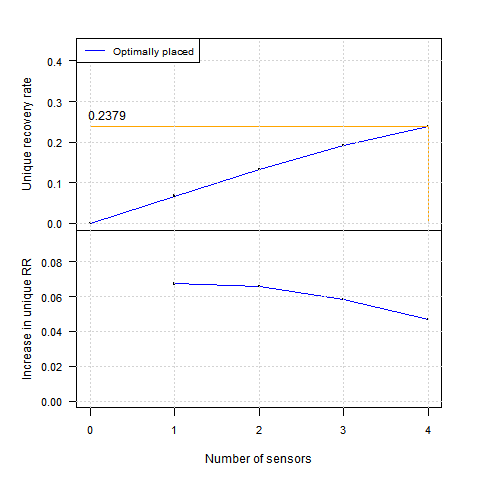
\includegraphics[scale=.7]{RecoveryRates.png}
	\caption{\label{recoveryGraph} A graphical representation of the cumulative and per-receiver UDRR.  User-placed receivers are representd by a grey line, system-placed receivers are represented by the black line, and projected receivers are represented by the green line.} 
\end{figure}

\subsection{Text Files}
The program returns a comprehensive text representation of the program output (text dump of gridded data and input parameters), and a short, human-readable document that lists the primary simulation parameters (Evaluation Algorithm, Suppression Algorithm, Behavioral Model, Input Grid Size, and Detection Range), as well as a tabular output of receiver placements (coordinates), data recovery rates for each receiver, and network sparsity.  Projected receivers are excluded from the total UDRR, ADRR, and sparsity values.

Coordinates are returned in both a Global (with respect to the original Topography file) and local (the user specified area of interest) frame.  While the curvature of the earth is well documented, different bathymetric maps may handle the mapping of a 3D curved plane to a 2D Grid differently.  For example, one Grid may implement some scaling on Grid cells a function of the cell's latitude or distance from a certain point.  Other Grid files may simply provide non-square Grid files.  By proving a small-scale (local) and large-scale (global) frame of reference for our receiver locations, irregularities of this nature are more easily detected.

\begin{figure}[ht]
	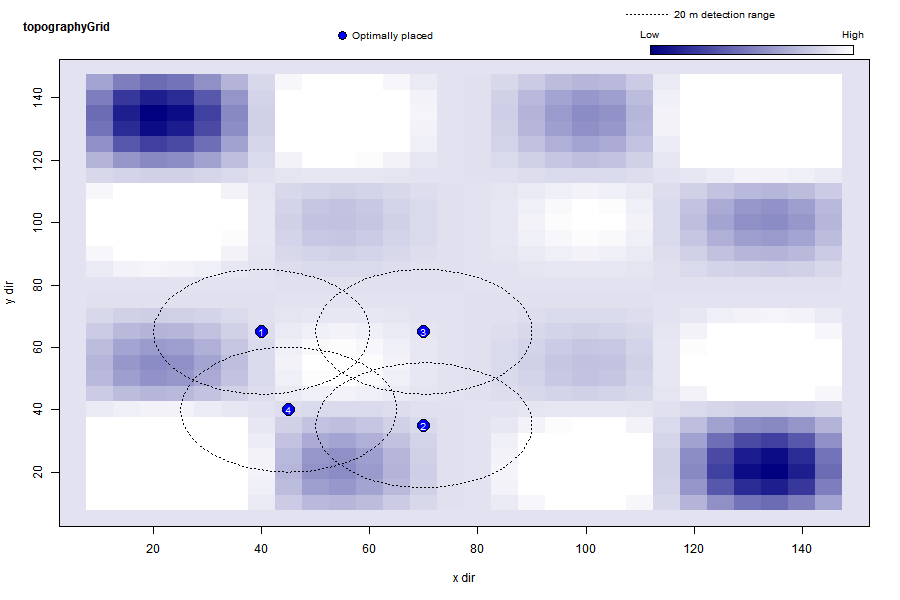
\includegraphics[scale=.5]{TopographyGrid.png}
	\caption{A graphical representation of an artificial Bathymetry file at a 1m resolution (each cell has an edge length of 1m).  Darker cells represent greater depths, while white cells represent inaccessible terrain (dry land).  The optimal receiver locations are shown on the Grid as blue numbered circles, user-placed sensors as grey circles, and projected receivers as green circles.  All receivers have their Detection Range shown as dotted lines.\label{bathyGraph}}
\end{figure}

\begin{figure}[ht]
	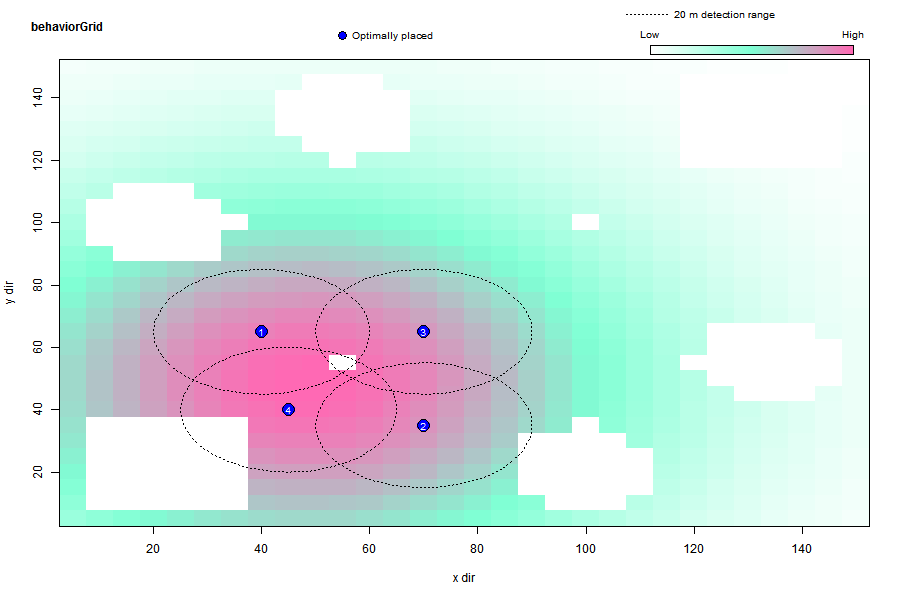
\includegraphics[scale=.5]{BehaviorGrid.png}
	\caption{The Behavior Grid represented as a heat map  Higher levels of animal residency correspond with pink cells, moderate levels as light blue, and white for non-residency (inhospitable habitat such as  dry land).  The optimal receiver locations are shown on the Grid as blue numbered circles, user-placed sensors as grey circles, and projected receivers as green circles.  All receivers have their Detection Range shown as dotted lines.\label{animalGraph}}
\end{figure}

\begin{figure}[ht]
	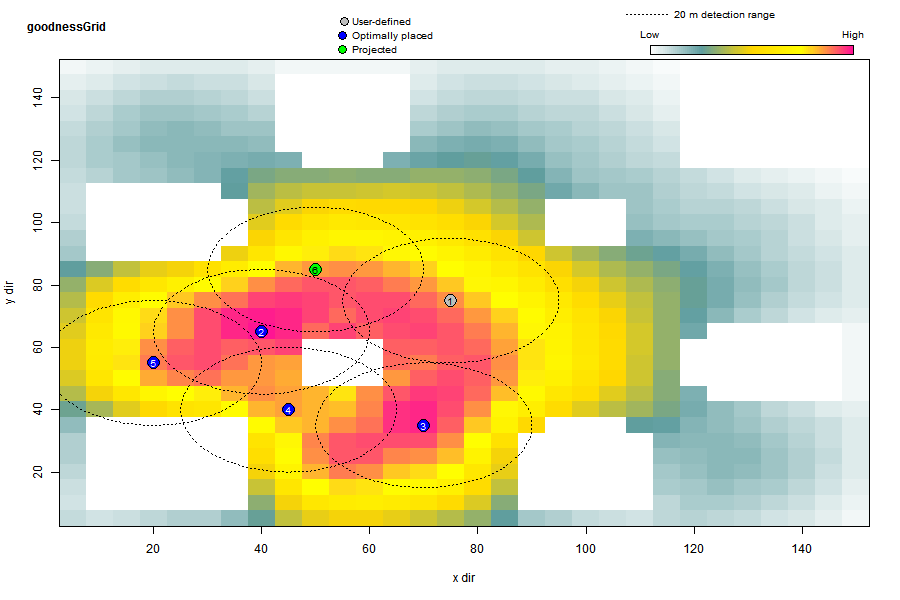
\includegraphics[scale=.5]{GoodnessGrid.png}
	\caption{The Goodness Grid represented as a heat map showing the sum total of Estimated Receivable Transmissions (ERT) for a receiver placed in a particular cell.  The legend in the top right assigns color coding to various ERT values. The optimal receiver locations are shown on the Grid as blue numbered circles, user-placed sensors as grey circles, and projected receivers as green circles.  All receivers have their Detection Range shown as dotted lines.\label{GoodnessGraph}} 
\end{figure}

\begin{figure}[ht]
	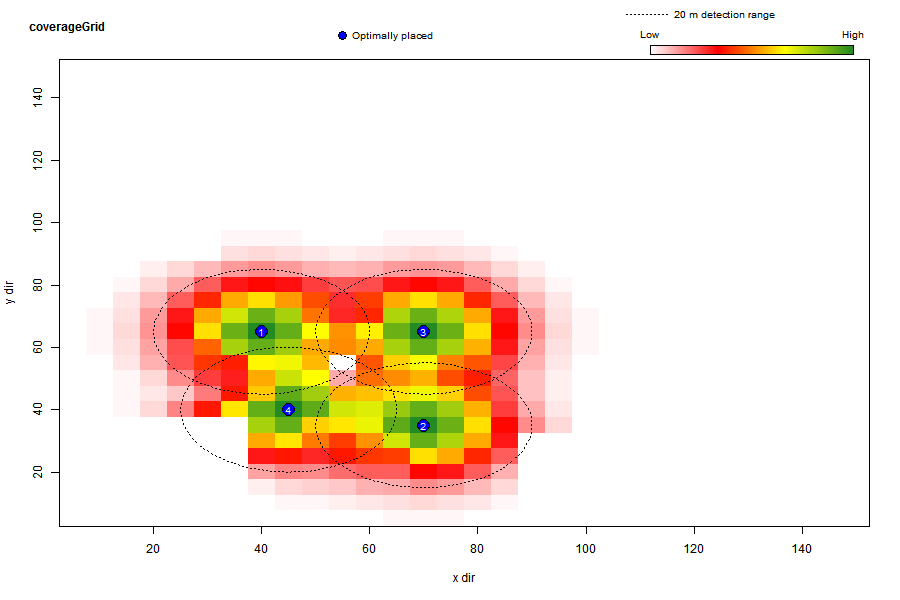
\includegraphics[scale=.5]{CoverageGrid.png}
	\caption{The Coverage Grid represented as a heatmap showing the quantity of Estimated Receivable Transmissions from each cell in the study site, for the designated receiver array configuration.  The legend in the top right assigns color coding to various ERT values.  The optimal receiver locations are shown on the Grid as blue numbered circles, user-placed sensors as grey circles, and projected receivers as green circles.  All receivers have their Detection Range shown as dotted lines.  The missing corner of of Receiver 4's Detection Area is due to the presence of an obscuring section of Bathymetry (dry land).\label{coverageGraph}}
\end{figure}
	
\section{Distinguishing Characteristics}
The challenge of acoustic network design is one that is common within the acoustic tracking community, yet rarely addressed.  While there are many methodologies, applications, and services that focus on achieving various objectives, this framework distinguishes itself in its availability, and adaptability.  

\subsection{Availability}
As previously stated, our framework is freely available \cite{acousitcdeploy} and falls under the GNU General Public License (GPL 2).  This availability means our methodologies are open-sourced, fully transparent, and are available for peer-review.  Furthermore, our framework is accessible to researchers without requiring expertise in R.  The web application provides a useful set of well-documented functionalities with a user-friendly interface.

\subsection{Adaptability}
\subsubsection{Flexability}
Many of the modules in this framework can be used as stand-alone functions that perform useful operations (reading bathymetric data, calculating distribution densities, etc).  This modularity allows the framework to function more like a library for acoustic simulation than a fixed application.  

\subsubsection{Simple Data Formats}
Many key functionalities of our framework (Evaluation Algorithms, Suppression, Animal Modeling, Network Statistics) operate over very simple data containers (Grids).   This simplified data format makes it easy to import, export, and convert between other data formats.  This simplified format also makes it easy to move data between this framework and other R packages.

\subsubsection{Customizable}
While other applications and methodologies optimize for fixed-objective functions (k-neighbor coverage, fixed detection probability, etc), our framework allows for user-customized objective (''Goodness'') functions.  Section~\ref{dispatcherFunctions} discusses dispatcher functions, which serve as abstract entry points into stand-alone modules, and allow highly-customized sub-functions to be aggregated together into uniform modules.  These dispatcher functions makes it easy to integrate new functionality into the framework without affecting other sub-functions.  

\subsection{Drawbacks}
\subsubsection{Explicit Data Validation}
In most all software systems, future efforts to add new functionality require a different set of parameters than those initially specified.  Thus, future developers will likely need to modify function signatures to incorporate said functionality.  This modification can substantially impact the way users interact with the system, and will require other developers to become familiar with a modified interface.  Additionally, these changes can potentially break older functions that relied upon the old function definition.  To reduce this brittleness (a small change causing a system to break) associated with explicit parameters, we utilize dictionary-based parameter passing.  While explicit parameters cause brittleness within a system, they serve to create a contract between users and functions, such that if users provide those explicit parameters, the function will operate as intended.  This contract is enforced by the programming language, resulting in compilation/interpretation errors when these parameters are violated.  Without explicit parameters, this contract is gone, and the responsibility of enforcing the relationship (by way of key-value validation within the dictionary) between users and functions falls to either the user or the developer.  In short, dictionary-based parameter passing provides reduced brittleness and simplified future-development but passes the responsibility of data validation to users and developers.

\subsubsection{Technical Capability}
While a fully functional application is provided as a demonstration of this framework, the framework's greatest usefulness to a tracking project will likely not be realized unless custom Goodness functions are defined.  Because substantial expertise in programming is required to author these custom functions, the framework is less useful to users with little R experience.  

\subsubsection{Language Limitations}
This framework was implemented in the R programming language primarily due to its popularity within the biological community.  While R is sufficient for small and medium scale simulations, a compiled language would offer significantly faster execution at all simulation levels.  Additionally, the R platform does not offer good support for reverse compatibility.  Specifically, R packages need to be recompiled under the local system's version of R.  If this compilation is unsuccessful (perhaps due to a difference in R versions, or operating system limitations), the package will not function.  If an application requires a significant number of R packages, then it is likely to be limited to operating within specific versions of R.

\section{Future Work}
\subsection{Emperical Analysis}
The analytical framework described herein is largely theoretical, despite a basis in well documented physical phenomena.  In order to better understand the correctness of our analysis, it would be useful to analyze empirical data from small-scale acoustic networks designed with this application.  Specifically, we are interested in the accuracy of our network coverage projections, and the affect of bathymetric resolution on this coverage.  

\subsubsection{Acoustic Coverage}
Recall that estimated data recovery rates are calculated based upon acoustic coverage and animal distribution.  While we provide basic Animal Models, the accuracy of these models (and as a result the accuracy of our data recovery rates) is very species-dependent and outside the scope of this paper.  While data recovery rates are based on animal models, our acoustic coverage model is not.  Thus, we are very interested in the accuracy and optimality of our bathymetric shadowing and network coverage models.  It would be interesting to compare the acoustic coverage of a real-world network designed by our application against our theoretical coverage of that same network.

\subsubsection{Bathymetric Resolution}
Section~\ref{bathymetyricModeling} describes the nature of artificially increasing bathymetric resolution.  It would be interesting to see how varying the native resolution of bathymetry affects the acoustic coverage of network topology both within our framework and in the real world.

\subsubsection{Workflows}
The workflows described in Section~\ref{workflows} were based upon both personal experience and imagined use.  It would be good to investigate the actual use cases, workflows, and problems that researchers face at various points throughout the lifetime of an acoustic tracking project.  By identifying unconsidered problems and workflows, the framework can be modified/expanded to encompass new roles and features, leading to greater usefulness.

\subsection{Heuristic Algorithms}
Recall that the function of the Goodness Grid is to store Goodness values for various locations within the study area.  The sample application simply computes every possible goodness value in the Goodness Grid, and then finds the top values Goodness values via R's $max()$ function.  While this process is guaranteed to find optimal receiver positions, it is computationally intensive, accounting for the vast majority of the program's run time.  Utilizing heuristic algorithms can significantly reduce the number of Goodness values that are computed, but can also reduce the optimality of the final acoustic array.  Heuristics are currently not included in the framework because functions involving Evaluation Algorithms and any new heuristic algorithms will likely be tightly coupled (a heuristic algorithm will likely need to consider an Evaluation Algorithm's definition of $Goodness$).  Furthermore, to avoid computational overhead (such as passing large lists of heuristic candidate cells), it is likely that the heuristic algorithm and Evaluation Algorithm will be called from within the same function.  This will likely lead to a large number of customized functions that implement heuristic algorithm-Evaluation Algorithms combinations.  It would be very useful to evaluate the cost of programatically de-coupling Evaluation and heuristic algorithms and passing large lists of heuristic candidates.  This data could then be compared against the measured benefits of various heuristic algorithms to evaluate the best methodology for integrating heuristics into the framework.  Another useful avenue would be the investigation of Evaluation Algorithm agnostic heuristics, which could provide better run times without tight couplings.

\subsection{Interactive Visualizations}
It could be useful to allow users to interact with the output graphs as a graphical user interface.  Users would able to move receivers around the graph and see how new placements affects network statistics in real-time.  Given that the Goodness Grid can be pre-computed, moving receivers and updating the effects of that movement in real-time requires very little re-computation.  In this case, it might be unnecessary to even pre-compute the Goodness Grid, but instead only preform the Evaluation Algorithm on cells where a user places a sensor.  This would allow users to quickly see how various receiver arrangements affect their network design, and facilitate rapid, impromptu prototyping of various configurations.  

Utilizing 3D visualizations could further enhance the user's understanding of network topology.  Figure~\ref{3d} illustrates a first-person view of the 3D environment modeled by the program.  Here, bathymetry is rendered as 3D mounds, with animal distributions represented by green fish, and receiver coverage by red spheres.  Users might be able to ''swim'' through the 3D environment, viewing their network from various angles.  Such a visualization would help users better understand what is being modeled, how their array is laid out, and where modifications might be helpful.

\begin{figure}[ht]
	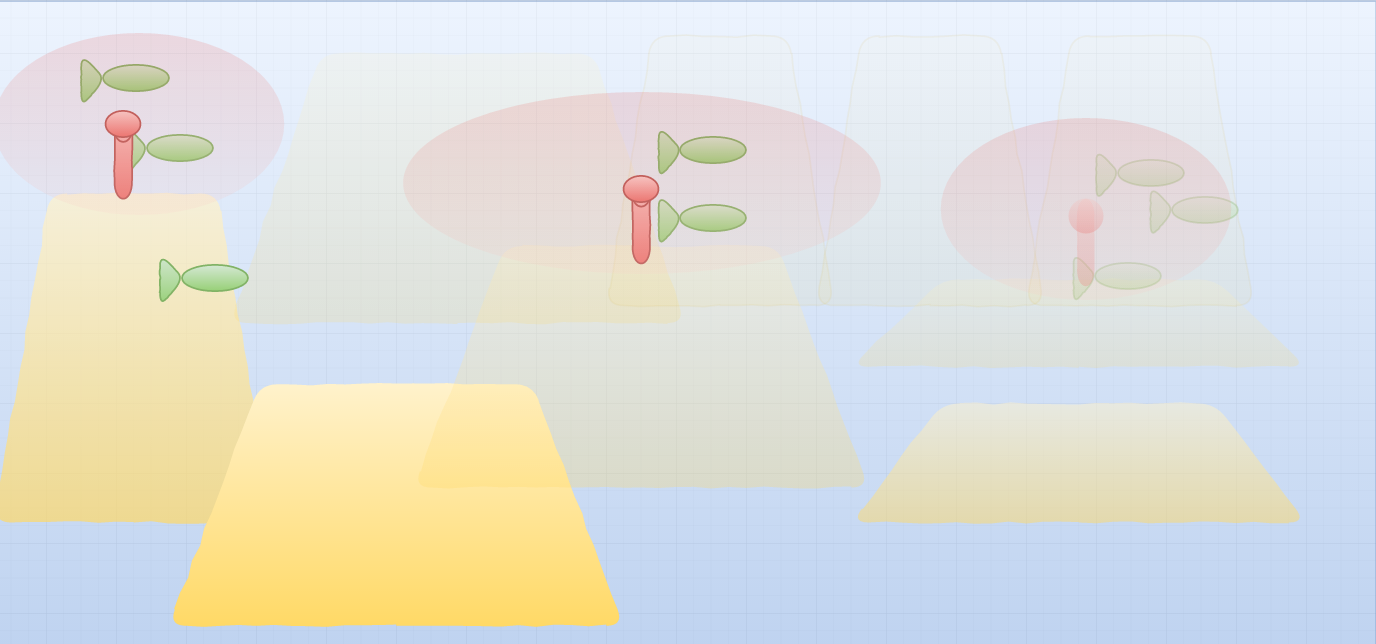
\includegraphics[scale=.45]{3d.png}
	\caption{A first-person view of the 3D space modeled in the program.  Users would be able to ''swim'' through the environment and gain a better perspective on what they are modelling, what their receiver array might look like in the environment, and where more receivers might be needed.\label{3d}}
\end{figure}
